\chapter{Real Time Impelementation}

In this chapter the real time implementation of the trained networks will be described. The main focus will be on integrating the model into an environment where it can process the incoming data in real time and provide estimations with as little latency as possible. 

\section{Development Environment}

Before describing the development environment, the meaning behind real time implementation should be clarified. In this context, real time means that the model is able to process incoming data and provide estimations within a fixed time frame, which is determined by the system. Within every defined time step, the computational unit (eg. microcontroller) receives new input data at the beginning of the time step, processes it using the implemented model, and outputs the estimation before the next time step begins. This setup can be seen on figure \ref{fig:rt}

\FloatBarrier
\begin{figure}[h]
    \centering
    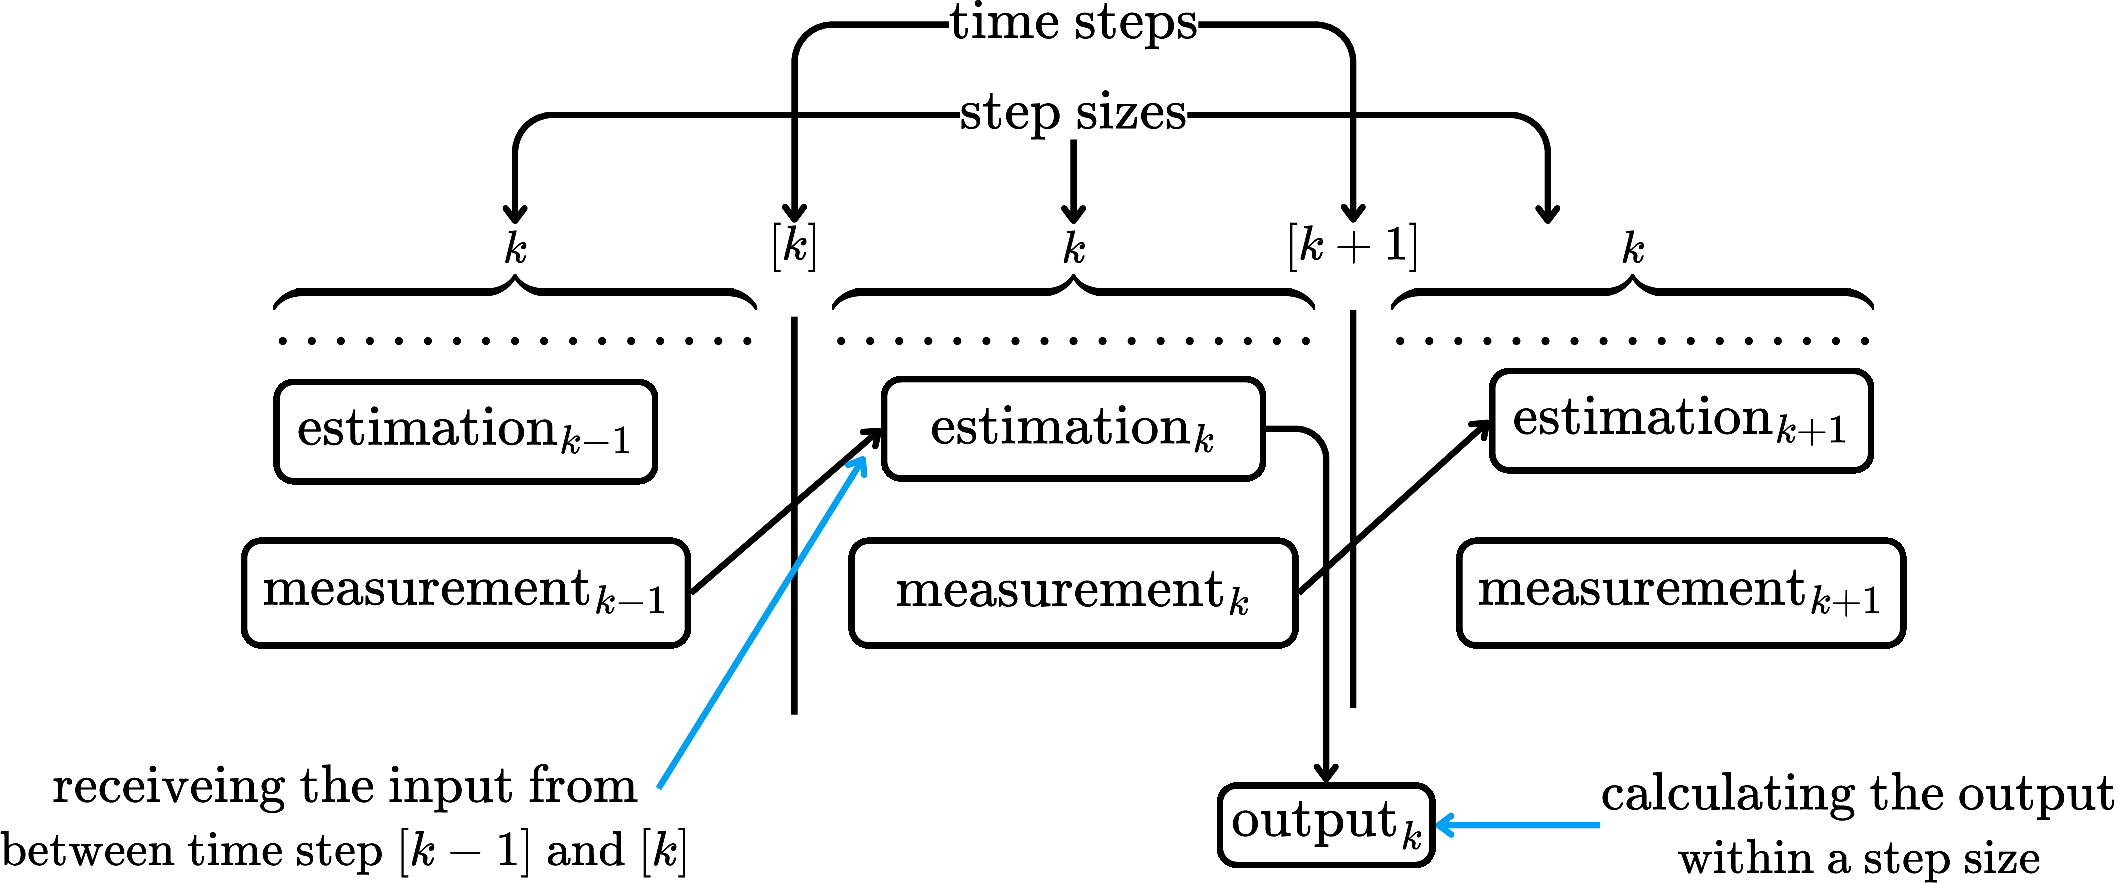
\includegraphics[width=0.9\textwidth]{images/rt.pdf}
    \caption{Real time implementation concept}
    \label{fig:rt}
\end{figure}
\FloatBarrier

A possible development environment for implementing an arbitrary control or estimation algorithm for vehicle application can be a toolchain offered by dSpace. This toolchain allows the user to create models in MATLAB Simulink, generate C code from these models and utilize the generated code on the hardware developed by dSace, where it can be tested in real time. The hardware can be connected to a real vehicle via the CAN bus, or to a simulator for cost efficiency reasons. In this thesis the latter application was chosen, using the BeamNG.drive simulator. The main steps of the real time implementations are the following:
\begin{enumerate}
    \item Prepare the trained models in MATLAB using the Deep Learning Toolbox (DLT).
    \item Integrate the trained models into MATLAB Simulink using DLT.
    \item Generating C code from the Simulink model using dSpace's ConfigurationDesk software.
    \item Deploying the generated code on dSpace's MicroAutoBox hardware using ControlDesk software.
    \item Connecting the MicroAutoBox to computer that runs BeamNG.drive via CAN bus.
    \item Testing the real time performance of the models with different step sizes.
\end{enumerate}
The toolchain of the real time implementation is illustrated in Figure \ref{fig:rt_toolchain}.
\FloatBarrier
\begin{figure}[h]
    \centering
    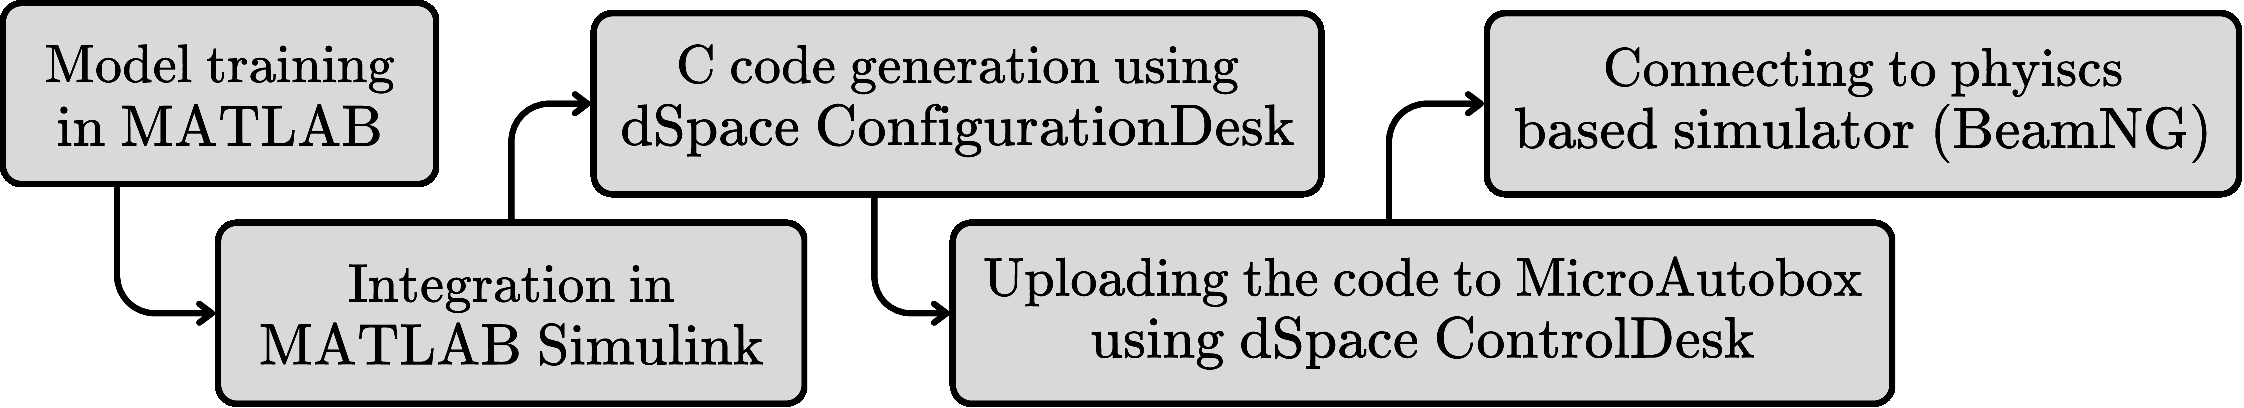
\includegraphics[width=0.9\textwidth]{images/rt_toolchain.pdf}
    \caption{Toolchain of the real time implementation}
    \label{fig:rt_toolchain}
\end{figure}
\FloatBarrier
The main question to answer is what is the smallest step size that the MicroAutoBox requires to be able to run the model. In other words, how much time does the MicroAutoBox need to process the inserted model and provide and estimation. This is crucial question since the smaller the step size, the more accurate and responsive the estimation will be, which can result better overall performance in a control application. 

\section{Results}

The chosen models for real time implementation were the best performing LSTM, GRU and the TCN architectures described in Chapter \ref{ch:direct_estimation}. Before starting the tests, a short calculation was made to estimate the FLOPS (floating point operations per second) required by each model. This gives a rough idea about the computational requirements of the models, which can be compared to the capabilities of the MicroAutoBox hardware. The calculated FLOPS are the following:
\begin{itemize}
    \item GRU:
\end{itemize}
\begin{equation}
    \text{seq len} \times \text{hidden size}^2 \times \text{layers}\times \text{gate factor} = 90 \times 208^2 \times 3 \times 6 \simeq 70.088 \text{ MFLOPS}
\end{equation}
\begin{itemize}
    \item LSTM:
\end{itemize}
\begin{equation}
    \text{seq len} \times \text{hidden size}^2 \times \text{layers}\times \text{gate factor} = 50 \times 192^2 \times 2 \times 8 \simeq 29.491 \text{ MFLOPS}
\end{equation}
\begin{itemize}
    \item TCN:
\end{itemize}
\begin{equation}
    \text{seq len} \times \text{channels} \times \text{kernel}\times \text{layers} \times \text{conv per block} = 50 \times 64 \times 4 \times 4 \times 2 \simeq 0.012 \text{ MFLOPS}
\end{equation}

The results indicate that the TCN model has significantly lower computational cost compared to the recurrenet models which makes it even more desirable for real time applications.

In table \ref{tab:rt_comparison} the highest task turnaround times that were read out on the MicroAutoBox are indicated for the specific models and an adivsable minimal time step for each model.

\begin{table}[h]
    \centering
    \begin{tabular}{|c|c|c|}
        \hline
        \textbf{Model} & \textbf{Max. turnaround time [ms]} & \textbf{Advisable min. step size [ms]} \\
        \hline \hline
        LSTM & 68.4 & 100 \\
        \hline
        GRU & 124.5 & 200 \\
        \hline
        TCN & 25.8 & 50 \\
        \hline
    \end{tabular}
    \caption{Real time implementation results on dSpace MicroAutoBox}
    \label{tab:rt_comparison}
\end{table}

After measuring these step sizes, it is clear that the TCN model is the most suitable for real time application due to its low computational cost and high accuracy. The main difference between the RNN based models is the sequence lenght which greatly affects computational costs. The LSTM model has a sequence length of 50 while the GRU model has a length of 90, which results in almost double the computational cost for the GRU model despite having only one layer more than the LSTM model.